% chapters/ch04.tex —— 第 4 章
% 体例：具体失败 → 设计问题 → 机制解释 → 对照实验 → 条件变化 → 选择原则
% 数字身份纪律：2607.07663 / 2608.03392 的数字一律 \cited{}；
% E02 运行 E02-20260924T153511Z-421eac 的数字一律 \measured{}；
% 由实测数字算出的倍数与差值用 \calcnum{}。
\chapter{从运行轨迹到可信反馈}
\label{ch04}

\chaptergoal{系统应该从一次失败中学到什么？}
\chapterprops{P2b 的现有数据与设计缺口。E02 保留为六种完整方案的试验记录，
不能代表形式证明到内在信号的完整层级；P2与P2b分别提出因素贡献和反馈作用条件的问题。}
\chapterfig{图~\ref{fig:ch04-ladder}：定性验证层级与 E02 的实际比较范围}
\chapterpitfall{模型读到了测试断言，却把“读取栈顶”解释为“弹出栈顶”；后续诊断正确也不等于修改已经发生。}

% ---------- 1. 具体失败 ----------
\begin{failurebox}
E02 的训练题 \texttt{classstate-02} 要求实现一个栈。原始代码的
\texttt{pop} 方法在非空时返回 \texttt{self.items[-1]}，没有删除元素。
在自评臂的任务轨迹中，Agent 读到了源文件和测试文件；测试明确要求先压入两个元素，
再弹出一次，此时内部列表只剩第一个元素。它却解释说已有代码已经“删除并返回”栈顶，
没有写文件就结束了任务。实验台记录的最终验收为未通过。

随后，归档经验写对了问题：“实现 pop 时既要返回栈顶，也必须删除该元素，否则 items 不变；栈空才返回 None。”
这句话出现在任务结束后的记忆里，没有回头修复刚才的提交。
同一臂的训练反馈标签与验收标签 \measured{8} 条全部一致，
而封存题回合通过率是 \measured{0.6125}，无记忆基线为 \measured{0.8125}。
这两个层面的记录可以同时成立：\textbf{结果标签对得上，并不说明诊断已被执行，更不说明经验能迁移。}

本例可直接核对任务轨迹与归档经验。中间那次模型自评的原始文字没有单独保存，
因此不能把经验句冒充自评原话，也不能由封存成绩倒推它导致了多少失败。
\end{failurebox}

\designquestion{一次失败能给出的东西有三样：一个标量结果、一段可重放的过程、
一个别人的判断。本章的问题是：\textbf{这条信号在什么条件下能被兑换成能力变化}，
以及当兑换没有发生时，我们靠哪个量把“信号不够好”和“信号没被用好”区分开。}

第 3 章立了协议，第 5 章起讨论经验写成什么样。本章夹在中间，处理的是更靠前的一段：
轨迹里本来就有很多信号，但它们回答的是不同问题：有没有达到要求、哪里值得检查、
为什么会出错、下一步该改什么。把这些问题压成一个“反馈质量分”，往往会把证据链中断的地方藏起来。
本章沿着一份真实记录拆开这些环节，再讨论怎样设计可识别的反馈比较。
验证层级是整理信号来源的定性视角，不是已经得到证明的收益上限。

% ---------- 2. 机制解释 ----------
\section{沿着一份栈实现，把反馈拆成可检查的对象}
\label{sec:ch04-stack-case}

章首案例值得展开，因为它的失败不需要猜测模型的内心。我们能看到模型收到的文件、实际调用的工具、最后的提交和归档经验；这些记录已经足以定位几处不同的断点。以下以自评臂为主，横向参照同题其他臂。没有归档的中间评审文字保持缺失，不用事后生成的解释补齐。

\subsection{要求的是状态变化，模型解释的却只是返回值}

一个栈的弹出操作有两个可观察结果：调用者收到什么，栈内部剩下什么。题目中的错误实现只完成前一项。若栈内依次放入元素 $a$ 和 $b$，读取末项会返回 $b$，但内部序列仍为 $[a,b]$；真正弹出后应当剩下 $[a]$。空栈返回什么则是第三个分支，不能代替非空时的状态检查。

原始测试恰好把这几个方面拆开了：一个用例看返回的栈顶，一个用例看弹出后的内部列表，还有一个用例看空栈返回值。因此，这次错误并不是现有测试完全漏掉了状态变化。自评臂实际读取的测试文本中已经包含内部列表的断言。模型随后给出的完成解释，却把代码里不存在的删除操作描述成已经存在。

这提供了一个比“模型不会写栈”更精确的诊断：\textbf{模型将函数名所暗示的语义，错误地投射到了当前函数体上。}这是根据可见文字与代码不一致所作的解释，不是对模型内部表征的测量。检查记录时应保留这个层次差别。我们可以确认它声称删除、实际上没有删除；至于产生这种错读的内部原因，现有轨迹不能唯一确定。

从工程上看，反馈应把注意力拉回缺失的状态转换。只说“栈实现有错”太宽；只说“第二个测试失败”仍要求执行者自己定位；指出“返回末项后列表长度没有减少”则直接给出一个可验证的局部假设。下一步修改也由此变得具体：在非空分支执行删除并返回被删元素，同时保持空栈的既定返回约定。

这里的正确性还依赖任务契约。若接口要求的是查看栈顶而不修改容器，那么读取末项完全合理。不能把本例的教训缩成“末项索引是错误写法”再用于所有容器接口。值得保存的是操作的后置条件，而不是对某个代码片段作永久的好坏标记。

\subsection{实际轨迹没有执行它声称完成的修改}

该回合的记录中没有写文件操作。Agent 先列文件，再读取源代码和测试，最后结束。模型某次回复同时写了两个读取请求，但旧解析器只执行匹配到的第一个；下一轮才实际读到测试。这也提醒我们，不能把模型输出里出现的工具请求一律算作已经发生的动作。

轨迹分析至少要区分请求、接受、执行结果三层。模型写出一行调用，只能证明它提出了请求；工具结果表明调度器怎样处理；工作区的文件内容或后续验收才支持动作产生了什么效果。若只抓取模型文字来构造“行为序列”，这里就会平白多出一次已执行读取。类似地，模型说“已修好”没有任何权限替代文件差异。

这段记录中，可读测试、错误解释和未修改提交发生在同一个任务回合；任务结束后的自评与经验生成属于另一阶段。归档经验指出缺失删除，说明后续文本中出现了正确的局部规则。它不能证明前一个回合经过了修复，也不能证明这条规则来自某一句特定的自评，因为那次自评原文没有保存。

把阶段划清以后，所谓“系统已经知道答案却仍失败”就不再神秘。知道的时间不同，持有这条信息的组件不同，允许采取的动作也不同。当前回合已经封账，经验写入器只产生下一题可读的文本；没有回到当前工作区的修订分支，就不会改变这次提交。是否加入修订分支，是下一版流程的设计选择，并非在报告里补写一句反思就能实现。

\subsection{同题其他臂提供的是参照，不是反馈质量的纯比较}

在同一道栈题上，五个反馈臂的训练验收都为未通过。测试判定臂、评审提示臂和自评提示臂都出现了对原实现的错误肯定；执行输出臂的末尾还出现无法按正常结束格式解析的文本。这些细节说明，最终失败可能经过不同路径，不能只看“未通过”三个字就归并为同一原因。

五条归档经验都指出应当删除栈顶。它们的措辞相近，却不能证明五种反馈通道等价。首先，这是失败以后写下来的经验，未直接测试经验驱动的当前题修复。其次，各臂此前的经验不同，提交与上下文未固定。再次，模型评审的输入、纯执行输出的输入和带标签的输出在信息量上并不匹配。一个任务上的相同终点，可以由不同的过程到达。

若想把这道题变成严格的反馈比较，第一步应冻结同一份错误代码和同一份题目说明。第二步才将不同反馈交给从同一状态开始的修复者。第三步用不参与提示构造的检查评估修改后版本，并记录修复耗时、调用与新增错误。这样估计的是“在这类已知错误提交上，给某种反馈对修复的影响”。它与原 E02 的“训练并积累经验，再到封存题作答”是两个不同问题，应分别运行和报告。

我们还做了不调用模型的本地行为复核：让错误方法与符合题意的候选方法接受同一组操作，比较返回值和容器状态。原方法返回末项后保留两个元素，局部修改后仅留首项，空栈行为保持不变。这验证了本例的状态差异，却不会产生“Agent 学会了修复”的实验证据。局部语义复核、模型修复效果与跨任务迁移，不能共用一个成功标签。

\subsection{一条可用的反馈记录应该保留什么}

从本例出发，可以构造一张用于诊断的记录卡。以下字段是本书建议，不是声称历史 E02 已完整实现的格式。记录卡先指向任务与候选代码版本，然后存放原始观察：某次操作之后返回什么、状态是什么、哪个断言没有满足。解释字段另写“可能缺少删除操作”，修改假设字段写“执行删除后，列表长度应减少且返回原末项”。最后注明验证范围与仍未检查的分支。

原始观察和解释分开存，有两个用途。其一，解释被推翻时还能回到未改写的证据；其二，不同诊断器可以读取同一观察，比较谁提出了更有效的修改。如果只保存一句“栈操作要正确维护状态”，下游既不知道这句话来自实际失败、作者常识还是模型猜测，也无法检查它是否遗漏了空栈行为。

记录卡不必把整段聊天复制到每一次提示。完整原文可以在证据库中保留引用，提示内仅呈现当前判断需要的片段。压缩时却应保持关键对应关系：哪个版本、哪个输入、哪个观察、哪条假设。长度预算紧张时，优先删掉礼貌话与重复说明，而不是把失败分支和适用条件一起删掉。

\section{从结果到修改：四个不同的准确性问题}
\label{sec:ch04-four-links}

“反馈准确”常常把四件事混在一起：结果标签是否匹配检查器，解释是否符合轨迹，建议是否能修复当前候选，经验是否有益于未来任务。它们处在不同位置，需要不同的分母。若不先分开，系统很容易在最容易度量的一层表现良好，然后把成绩转借给其他层。

\subsection{标签一致性检查的是判定，不是更新}

设一次候选的检查器结果为 $y$，反馈文本明确给出的成功指示为 $\hat y$。比较 $\hat y$ 与 $y$，可以得到这批有可解析标签的反馈中有多少不一致。这个量不需要系统真的修改代码，也不需要经验进入经验库。即使所有经验都被删除，标签不一致率仍然能够计算。因此把它命名为“错误更新率”，会让读者以为我们检查过更新行为及其后果。

如果反馈没有明确标签，不能为了方便统计就自动填成失败。缺失可能来自格式错误、保留意见、无法判断或根本没有要求输出标签。应报告标签覆盖率，并在可判定部分计算一致性；必要时按缺失原因分组。否则一个谨慎的评审者会因拒绝猜测而看起来更差，一个永远肯定的评审者反倒显得完整。

检查器标签也不是无需说明来源的真理。单元测试标签表示是否通过该组测试；人工验收表示是否满足该次验收约定。若二者不一致，首先要问它们是否检查同一目标，不能立即把一个命名为真值、另一个命名为噪声。E02 的对照真值限定为本实验台的验收结果，并未声称覆盖全部程序语义。

\subsection{解释相容性要求落到可见证据}

一段解释可以给对最终标签，却说错原因。比如程序失败是因为把传入的默认值硬编码掉，反馈却说需要捕获一种题目不涉及的异常。两个解释都能以“未通过”结尾，只有前者直接对应现有失败路径。检查标签不能发现这个差别。

因此应让诊断引用具体证据：某次输入、某个返回值、某条代码路径，或某个工具结果。引用本身仍不保证因果正确，但至少让解释可以被逐项反驳。若诊断说“函数修改了输入列表”，就可以检查调用前后的对象内容；若诊断说“检索选错了资料”，就需要列出被检索材料与题目要求的冲突。无法指出支持材料的诊断，应作为待查假设，而不是已定位故障。

还要容许证据不足。复杂任务的最终日志可能只说明请求失败，没有保留失败之前的状态。此时最合理的下一步可能是增加观测，而不是立即提出修复。把所有反馈模板都规定成必须给一个原因，会迫使系统把未知包装成肯定句，也使后续经验库积累大量不可追溯的解释。

\subsection{建议有效性需要实际干预}

要证明一个建议有帮助，至少需要观察按建议修改以后发生了什么。栈案例中把返回末项改成弹出末项，是一个局部可检验的干预；若同时重写构造器、改接口、替换容器并改测试，再看到通过，就无法把收益归到删除操作这一条建议。

工程修复未必总能只改一处，但报告应把联合修改说清楚。可以把最小修改与完整改写分成不同候选，先验证它们各自满足哪些断言。若多个候选都通过，运行成本、接口兼容与未覆盖行为也可能不同。测试结果给出当前覆盖内的证据，并不会自动替我们选出唯一最佳实现。

一个有用的反事实检查是：保持同样的初始提交与资源，只拿掉这条建议，修复者是否也能解决？如果没有这个对照，一次成功修复只能说明完整流程奏效，不能把全部改进归功于反馈文本。反过来，一次失败修复也可能源于预算耗尽或格式解析，未必表明建议内容错误。

\subsection{迁移收益要求回到目标任务分布}

经验用于下一题时，任务、输入或环境已经变化。局部规则是否仍适用，要由新的条件决定。对普通栈，“删除并返回”是弹出操作的要求；对不可变数据结构，接口可能返回一个新栈与元素；对只读视图，根本不允许改变内部状态。丢掉接口条件的经验越简短，越可能看起来普遍而实际上越界。

迁移评估应同时记录经验有没有被检索、有没有被采纳，以及采纳后相对无经验或替代经验发生什么变化。只统计经验命中次数，会把“经常出现”误作“经常有效”；只统计引用文字，又可能错过模型没有显式引用但受其影响的情况。可观察的使用痕迹有价值，但最终效果仍须通过适合问题的对照来估计。

这四层之间没有简单的乘法关系。一次粗糙但指出关键方向的反馈可能帮助修复，一条完全正确却不相关的知识也可能占用上下文。设计者需要知道每项指标在链条中的位置，而不是先合成一个总分，再凭总分决定全部更新。

\subsection{把发布门槛放在合适的位置}

可采用分阶段处理：原始观察进入证据库，未经验证的解释进入候选区，局部修复经过检查后形成带条件的经验，再由迁移观察决定是否广泛启用。这里的阶段不是越多越好，而是避免一种证据尚未具备时就赋予过大的决策权。

低风险提醒可以允许较低的证据门槛，例如提醒检查空输入；会自动改写代码的技能则需要更强的适用性与回归证据。二者若共用“置信度高即可发布”的规则，提醒文本就可能被误升级为可执行权限。第 6 章会讨论决策权，第 8 章会讨论技能准入；本章给出的依据是反馈证据的范围，而不是经验文字的语气。

发布以后也应保留回退路径。新的失败可能推翻原先过宽的适用条件，而不推翻经验的全部内容。处理方式可以是缩小范围、增加反例或降回候选区。若每次失效都整条删除，系统会丢失为何曾经认为它有效的历史；若从不降级，已知限制又无法影响执行。


\section{三种反馈粒度：结果、过程与偏好}
\label{sec:ch04-grain}

\begin{table}[htbp]
\centering
\caption{三种反馈粒度：它们给出的信息量、信用分配跨度与典型用途}
\label{tab:ch04-grain}
\begin{tabular}{>{\raggedright\arraybackslash}p{2.0cm}>{\raggedright\arraybackslash}p{4.4cm}>{\raggedright\arraybackslash}p{2.6cm}>{\raggedright\arraybackslash}p{3.4cm}}
\toprule
粒度 & 它给出什么 & 信用分配跨度 & 典型用法 \\
\midrule
结果反馈 & 一个标量：这次通过与否、得分多少 & 整条轨迹；不直接定位步骤 & 用验收结果筛选候选，或作为生成反思的输入 \\
过程反馈 & 若干位置的观察：回溯、异常、日志、资源曲线 & 可指向步骤；根因仍待查 & 定位故障，形成局部修改假设 \\
偏好反馈 & 候选之间的相对排序 & 指向候选；未必定位内部动作 & 在同一要求下比较候选，再用于选择或训练 \\
\bottomrule
\end{tabular}

\begin{minipage}{0.92\linewidth}
\vspace{2mm}
{\footnotesize 表注：本表按反馈表达的对象分类，用途为本书设计示例，不是三篇论文与三类信号的一一对应。一个实现可以同时使用多类反馈。}
\end{minipage}
\end{table}

三种形式没有统一的强弱顺序，也不能按方法名直接归类。
Reflexion 的评估结果可以先作为标量，再被语言反思模块转成诊断；Self-Refine 的反馈是可包含多方面建议的自然语言，不宜仅因发生在一轮输出之后就叫标量结果反馈\cite{reflexion-2303,self-refine-2303}。

\begin{samepage}
DSPy 可以通过给定度量筛选示例并比较候选，但“根据分数选优”不等于只获得两候选之间的相对偏好\cite{dspy-2310}。\par
\end{samepage}

要登记的是实际输入输出中有哪些信息，而不是给每套框架分配一个互斥标签。
标量结果所需记录很短，取得这个判定却未必便宜；它的信用分配跨度仍覆盖整条轨迹——
一次失败到底是第 3 步选错了工具，还是第 12 步把返回值写错了，标量不会告诉你。
过程反馈可能缩小排查范围，前提是保留了能与步骤关联的中间观察。
异常位置未必就是根因，日志也未必覆盖造成结果的全部状态；一个只返回最终分数的接口则没有直接提供这些观察。
本节所说的成对偏好反馈\textbf{只提供相对排序}：
它只能回答“这两个里哪个更好”，因此它天然需要一个候选生成器配套，
候选池或比较标准改变时，偏好胜率的变化不能直接解释为同一目标下的绝对质量变化。

本章后面所有讨论都默认一件事：
无论哪种粒度，\textbf{反馈必须有来源}。
来源决定了它能不能被重放、能不能被审计、以及它会不会在被优化的过程中变形。

\section{三个来源：执行测试、环境状态与模型评审}
\label{sec:ch04-source}

\begin{itemize}
  \item \textbf{执行测试}：把提交放进指定环境，检查给定断言。固定代码、依赖、输入与外部状态后可以尝试重放，
        但测试覆盖有限，时序和外部服务也可能使结果变化。测试通过不等于满足全部规格。
  \item \textbf{环境状态}：退出码、标准输出、异常回溯、耗时与内存。
        它们提供过程证据，其中也可能含明确判定，例如断言失败及其期望值；不能一概称为“无判定”。
  \item \textbf{模型评审}：模型阅读候选产物后给出的判断。原始评审文本可以归档并重放给下游，
        重新调用评审模型则未必产生相同文字。判断受模型能力、提示、上下文与可见材料共同影响。
\end{itemize}

这三条里藏着本书的一条可操作分界。
一篇覆盖 \cited{65} 篇工作的编程域自进化综述统计了各工作使用的信号类型，
其中 \cited{75.4\%} 依赖可执行验证（测试、编译器、基准），
依赖编码轨迹的 \cited{52.3\%}、软件诊断的 \cited{49.2\%}、
仓库与产物信号的 \cited{20.0\%}、人类开发信号的 \cited{4.6\%}、
质量信号的 \cited{3.1\%}；
还有 \cited{10.8\%} 的工作\textbf{完全没有使用任何代码特有的信号}——
它们只靠通用奖励、模型裁判或非代码的交互轨迹，
即便它们的评测跑的是代码基准\cite{coding-survey-2608}。

\section{六类信号：一份可核对的清单}
\label{sec:ch04-six}

\begin{table}[htbp]
\centering
\caption{六类反馈信号：需要核对的条件、典型操纵路径与语料占比}
\label{tab:ch04-six}
\begin{tabular}{>{\raggedright\arraybackslash}p{0.7cm}>{\raggedright\arraybackslash}p{2.2cm}>{\raggedright\arraybackslash}p{3.3cm}>{\raggedright\arraybackslash}p{2.2cm}>{\raggedright\arraybackslash}p{1.6cm}c}
\toprule
代号 & 类别 & 例子 & 核对条件 & 操纵路径 & 占比 \\
\midrule
E & 可执行验证 & 测试、编译器、形式化检查 & 规格、环境与覆盖 & 改测试或利用泄漏 & \cited{75.4\%} \\
D & 软件诊断 & 日志、异常、依赖冲突 & 日志来源与完整性 & 伪造或漏报 & \cited{49.2\%} \\
T & 编码轨迹 & 自身编辑序列、工具调用链 & 提议与实际执行 & 选择性留轨 & \cited{52.3\%} \\
R & 仓库与产物 & 构建结果、代码结构、文档 & 版本与依赖 & 改被测产物 & \cited{20.0\%} \\
Q & 质量信号 & 运行时、资源、安全、可维护性 & 负载与指标定义 & 只优化代理量 & \cited{3.1\%} \\
H & 人类开发信号 & 评审意见、开发者编辑、偏好 & 原意见与背景 & 筛选有利意见 & \cited{4.6\%} \\
\bottomrule
\end{tabular}

\begin{minipage}{0.92\linewidth}
\vspace{2mm}
{\footnotesize 表注：六类的定义与占比取自 \cite{coding-survey-2608} \S 4.2 与 Figure 7
（\cited{65} 篇语料，多标签统计，故占比之和大于 $100\%$；
另有 \cited{10.8\%} 的工作不属于任何一类）。
“核对条件”与“操纵路径”是本书提出的检查问题，不是发生率、可靠性评分或原文统计字段；原文提供分类与占比。}
\end{minipage}
\end{table}

这张表有两个读法值得写进正文。

第一个读法是\textbf{分布的偏斜}。
超过四分之三的工作依赖 E，而依赖 Q 的只有 \cited{3.1\%}、依赖 H 的只有 \cited{4.6\%}。
它说明这批研究经常利用编程环境中的可执行信号，但占比本身不能分解方法效果的原因，
也不能证明某类信号必然最强。跨到其他领域时，应重新寻找与任务目标相连的证据，
例如文献原文、交易回执或用户明确纠正，并核对它们的覆盖范围。

第二个读法是\textbf{推广时的缺口}。
这六类是\emph{代码特有}信号的分类。
把它推广到一般 Agent（检索型问答、多步工具调用、长程办公流程）时，
必须补上非代码域的对应物：检索命中与引用可核查性、用户显式纠正、
业务指标的滞后变化、以及“这一步有没有被下游真正用到”。
这个推广是\textbf{本书做的，不是原文做的}，
因此表~\ref{tab:ch04-six}中的核对条件与操纵路径是本书补充的分析，
不能算作 \cite{coding-survey-2608} 的结论。

\section{信用分配：哪一步值得保留或修改}
\label{sec:ch04-credit}

反馈到达的时刻几乎总是晚于造成结果的那个动作。
一次 episode 有十几步，判定在最后一步给出，
于是“哪一步该改”这个问题必须靠某种分摊规则回答，而分摊规则本身是一个假设。

E02 的各反馈臂在每个训练回合结束后写一条经验，不做逐步因果归因。
封存阶段用字符二元组重叠检索前 \measured{2} 条经验，不使用任务族标签。
这种检索可能带入与当前题无关的提示，但是否发生、是否改变行为、是否导致失分，需要分别核对。
下面的分族表只呈现结果异质性，不能单独证明跨族误检索是原因。

\begin{table}[htbp]
\centering
\caption{测试判定臂相对基线的收益，按题族分解（封存集，每族 \measured{2} 道配对题）}
\label{tab:ch04-family}
\begin{tabular}{>{\raggedright\arraybackslash}p{2.6cm}cc|>{\raggedright\arraybackslash}p{2.6cm}cc}
\toprule
族 & 收益 & 方向 & 族 & 收益 & 方向 \\
\midrule
mutabledefault & \measured{$-0.4000$} & 退化 & dictmiss & \measured{$+0.2000$} & 改善 \\
classstate & \measured{$-0.2000$} & 退化 & recursionbase & \measured{$+0.1000$} & 改善 \\
offbyone & \measured{$-0.2000$} & 退化 & strindex & \measured{$+0.0000$} & 持平 \\
sortkey & \measured{$-0.2000$} & 退化 & errorcontract & \measured{$-0.1000$} & 退化 \\
\bottomrule
\end{tabular}

\begin{minipage}{0.92\linewidth}
\vspace{2mm}
{\footnotesize 表注：八族里五族为负、两族为正、一族为零（\calcnum{5/8}）。
每族只有 \measured{2} 道配对题，本表\textbf{只用于说明收益在族间反号}，
不支持稳定的族级效应判断；族级结论需要专门的族分层设计。}
\end{minipage}
\end{table}

在这批题上，同一套经验与检索流程给出的分族差值有正有负。总体均值回答既定任务混合下的平均表现，分族读数则帮助定位值得进一步检查的失效模式。是否限制某一族的经验使用，应结合该族的补充比较、回归检查与风险要求决定。

\section{错误归因、偶然成功与反馈噪声}
\label{sec:ch04-noise}

一次通过不等于教训正确。
一次 episode 里可能有若干个动作是错的，只是恰好没有触发失败分支；
写下来的“教训”于是把偶然成立的写法固化成了规则。
这类情况需要针对失效条件补充检查。同一题重复生成可以观察生成的不稳定性，
却不自动补上缺失的断言；把同一份错误测试重复执行，也不会得到规格外的反例。

E02 的噪声臂设定标签翻转概率 $\pi=\measured{0.30}$，本轮实际翻转 \measured{2/8}。
但保留实现只翻转反馈开头的判定，后面仍附原始测试输出。
因此它同时改变了标签一致性和信息冲突，不能解释为纯粹的、不可辨识的标签噪声。
随机种子的构造还用了 Python 的字符串散列；仅保留基础种子不足以保证跨进程复现翻转序列。

\begin{table}[htbp]
\centering
\caption{反馈本身的质量：机制量，不是效果量（训练期）}
\label{tab:ch04-quality}
\begin{tabular}{>{\raggedright\arraybackslash}p{3.0cm}ccccc}
\toprule
臂 & 条数 & 有标签 & 不一致 & 不一致率 & 解析失败 \\
\midrule
arm\_formal & \measured{8} & \measured{8} & \measured{0} & \measured{0.0000} & \measured{0} \\
arm\_exec & \measured{8} & \measured{8} & \measured{0} & \measured{0.0000} & \measured{0} \\
arm\_review & \measured{8} & \measured{8} & \measured{0} & \measured{0.0000} & \measured{0} \\
arm\_self & \measured{8} & \measured{8} & \measured{0} & \measured{0.0000} & \measured{0} \\
arm\_noise & \measured{8} & \measured{8} & \measured{2} & \measured{0.2500} & \measured{0} \\
\bottomrule
\end{tabular}

\begin{minipage}{0.92\linewidth}
\vspace{2mm}
{\footnotesize 表注：历史字段名为 \texttt{mismatch\_rate}，比较的是反馈成功指示与验收标签，
并未检测更新造成的损害。测试判定臂直接使用验收结果，执行输出臂的指示由实验台私下取退出码；
二者的零不一致率不是模型理解能力。评审与自评臂才解析模型判定行。}
\end{minipage}
\end{table}

评审臂的训练结果为 \measured{5} 成功、\measured{3} 失败，自评臂为 \measured{6} 成功、\measured{2} 失败；
各自 \measured{8} 条标签均与验收一致，不能扩展为全部任务上的准确率保证。
噪声臂减测试判定臂的收益差为 \measured{$-0.0500$}，
历史题级区间为 \measured{$[-0.2000,+0.1125]$}。
这两个反馈臂独立完成训练与经验构建，这个差值比较的是两套反馈方案；它没有固定同一组来源输出后只翻转标签。区间含零不表示噪声无害，也不消除标签与执行输出同时出现的设计问题。
分辨能力与样本结构、差值方差、干预强度和统计方法都有关，不能只归结为题数。

\section{从诊断到可检验的修改假设}
\label{sec:ch04-hypothesis}

一条经验要能被检验，至少要有三样东西：
\textbf{诊断}（哪里错了）、\textbf{适用条件}（什么情况下这条成立）、
以及\textbf{一个可检验的修改假设}（改了之后哪个量会动）。
带条件的经验条目在实践中已有明确形态——
KSI用 \texttt{applies\_when} 与 \texttt{does\_not\_apply\_when} 表达正反适用条件\cite{ksi-2607}。
本书采用这一检查思路，但不要求所有表示都使用相同字段名；关键是条件能否被读取、检查并影响调用决定。

E02 的经验记录有源题、源族和验收结果等元数据；部分文字也写了边界条件。
例如栈的经验明确说到“栈空才返回 None”。因此不能概括为“没有一条经验有适用条件”。
更具体的问题是：检索只读经验文本，没有独立的适用性判断；经验中表达的条件，也没有被逐条验证。
把条件写出来只是建立了一个可审查的对象，还需要检查条件是否足够、是否与任务契约冲突。

第 5 章将继续讨论经验如何表示、合并与淘汰。本章先把证据链的入口做好：
反馈必须指向明确的候选版本、观察与适用范围，诊断必须能导出可以被推翻的修改假设。

% ---------- 3. 对照实验 ----------
\section{验证层级：定性观察与本书的受限比较}
\label{sec:ch04-hier}

\begin{table}[htbp]
\centering
\caption{验证层级四层（引自 \cite{rsi-survey-2607} \S 5.2）}
\label{tab:ch04-hier}
\begin{tabular}{cl>{\raggedright\arraybackslash}p{4.6cm}>{\raggedright\arraybackslash}p{4.4cm}}
\toprule
层 & 信号 & 性质 & 例子 \\
\midrule
1 & 形式验证器 & 依赖规格与检查器假设 & 证明检查器、类型系统 \\
2 & 执行反馈 & 可靠但\textbf{不完全}；固定基准存在过拟合与投机风险 & 测试、编译器、基准 \\
3 & 学习式评审 & 依赖评审者及其可见证据，也可能成为优化目标 & 奖励模型、LLM-as-judge \\
4 & 内在信号 & 原文概括为低成本、易投机；具体须测量 & 置信度、自一致性、似然 \\
\bottomrule
\end{tabular}

\begin{minipage}{0.92\linewidth}
\vspace{2mm}
{\footnotesize 表注：原文明确声明这条排序是
``a qualitative pattern we observe throughout the corpus, \textbf{not a measured law}''。
本表据此保留定性解释。E02尚未覆盖完整四层，不能仅凭臂名完成层级检验。}
\end{minipage}
\end{table}

这里需要区分概念排序与实验操作。形式证明、测试执行、模型意见、置信度不是四个可以仅靠改臂名实现的处理。
只有实际的信息来源和检查机制对应上了，才谈得上检验完整层级。

\subsection{E02：六种反馈与记忆方案的实际实现}

E02 共保留 \measured{528} 个回合轨迹，六臂各有 \measured{8} 个训练回合、\measured{80} 个封存回合。
训练候选池虽有 \measured{16} 题，配额只取排序后的前 \measured{8} 题，覆盖四个族；
封存集则有八个族、\measured{16} 题。各反馈臂从自己的提交生成经验，训练途中已检索此前的经验，
因此比较的是逐渐分化的完整流程，并非固定同一批提交后只换反馈文本。

任务提示没有列出验收工具，全部轨迹也没有实际调用它；但共用执行循环仍能处理该工具名，
所以“本轮没有调用”与“实现禁止调用”必须分开。测试文件可读，指定写工具限制直接修改，但未实施完整进程写保护，
不能将封存题解释为对 Agent 隐藏验收断言的题。
评审和自评都使用同一个后端、新建的单条用户消息；差别主要是角色措辞，
自评请求并未继承做题时的整段上下文。按保留实现重建，输入中的文件集合包含测试源码，
因此没有执行结果不等于没有断言信息。原始中间请求未归档，重建不能替代运行时输入记录。
后文保留旧臂标识，中文名称按实际操作解释。

\begin{table}[htbp]
\centering
\caption{E02 六臂在封存集上的回合通过率与相对无记忆基线的收益}
\label{tab:ch04-e02}
\small
\begin{tabular}{>{\raggedright\arraybackslash}p{1.9cm}>{\raggedright\arraybackslash}p{1.9cm}ccc}
\toprule
臂 & 反馈操作 & 回合通过率 & 收益 & 收益 95\% 区间 \\
\midrule
arm\_base & 无反馈基线 & \measured{0.8125} & — & — \\
arm\_formal & 测试判定及输出 & \measured{0.7125} & \measured{$-0.1000$} & \measured{$[-0.2125,+0.0125]$} \\
arm\_exec & 删总结行的输出 & \measured{0.7000} & \measured{$-0.1125$} & \measured{$[-0.2625,+0.0500]$} \\
arm\_review & 评审提示 & \measured{0.7125} & \measured{$-0.1000$} & \measured{$[-0.2375,+0.0250]$} \\
arm\_self & 自评提示 & \measured{0.6125} & \measured{$-0.2000$} & \measured{$[-0.3875,-0.0250]$} \\
arm\_noise & 受控噪声对照 & \measured{0.6625} & \measured{$-0.1500$} & \measured{$[-0.3125,+0.0125]$} \\
\bottomrule
\end{tabular}

\begin{minipage}{0.92\linewidth}
\vspace{2mm}
{\footnotesize 表注：模型 \texttt{deepseek-flash}，温度 \measured{0.7}，
训练集配额 $E=\measured{8}$，封存集 \measured{16} 道 $\times$ 每题 \measured{5} 个重新开始的回合
（每臂 \measured{80} 次运行），协议所用 MDE 设计值 \calcnum{0.03}，重采样单位为题。
收益 = 该臂回合通过率减基线臂回合通过率，按题配对；区间为按题重采样的 95\% 自助区间。
原始记录 \texttt{experiments/runs/E02-20260924T153511Z-421eac/}。}
\end{minipage}
\end{table}

\begin{table}[htbp]
\centering
\caption{按原臂顺序计算的差值（同一运行）}
\label{tab:ch04-adj}
\small\setlength{\tabcolsep}{4pt}
\begin{tabular}{>{\raggedright\arraybackslash}p{4.0cm}cc>{\raggedright\arraybackslash}p{3.0cm}}
\toprule
臂间比较 & 点估计 & 95\% 区间 & 未呈预期正序（差值 $\le 0$） \\
\midrule
测试判定 $-$ 执行输出 & \measured{$+0.0125$} & \measured{$[-0.1125,+0.1375]$} & 否 \\
执行输出 $-$ 评审提示 & \measured{$-0.0125$} & \measured{$[-0.1375,+0.1125]$} & \textbf{是} \\
评审提示 $-$ 自评提示 & \measured{$+0.1000$} & \measured{$[-0.0500,+0.2625]$} & 否 \\
\bottomrule
\end{tabular}

\begin{minipage}{0.92\linewidth}
\vspace{2mm}
{\footnotesize 三个相邻差中有 \measured{1} 个为负。历史规则也计入恰好为零的差值，那种情形是持平。
另一个历史比较为自评提示减执行输出的收益差：
点估计 \measured{$-0.0875$}、区间 \measured{$[-0.2625,+0.0875]$}，包含 0。
这些区间与点估计只描述本次数据，不构成完整层级的支持或反证。}
\end{minipage}
\end{table}

\subsection{读数、精度与不可识别的问题}

五个有记忆臂相对无记忆基线的点估计都为负。
自评臂的历史题级自助区间没有跨零，其余四臂跨零。
这些是具体模型、任务和已实现流程下的读数；自评臂的单个区间也不是多重比较校正后的层级检验。
区间能描述抽样不确定性，不能修复反馈类型与概念层级不对应的问题。

自评减执行输出的题级配对差标准差为 \measured{0.3722}，
测试判定减自评为 \measured{0.3183}。
把这两个试验估计代入 $n=(1.96s/0.03)^2$ 并向上取整，得到 \calcnum{592} 与 \calcnum{433}。
它们是正态近似下区间半宽为 \calcnum{0.03} 的后续规划参考，
不是这次试验预先冻结的样本量，也不是保证检出三个百分点效应的功效计算。
样本标准差本身仍有不确定性；独立任务、同族相关、重复回合以及多重比较都应进入新的规划。
具体区别见附录 A。

回答P2b需要先使操作对应所讨论的反馈类型，并匹配任务覆盖与比较设计。
P2 还要求在统一循环中交叉操纵反馈与更新对象。
拿 E01 与 E02 的跨度相减、标准化或求比值，都不能消除两项实验之间的流程差异。

\begin{figure}[htbp]
\centering
% Quantitative panel generated from archived E02 data; provenance in calculations.
\begin{minipage}{0.96\linewidth}
\centering
\begin{tikzpicture}[r/.style={draw,rounded corners=2pt,text width=30mm,align=center,font=\small,minimum height=14mm}]
\node[r] (a) at (0,0) {形式验证\\依规格与检查器};
\node[r] (b) at (3.7,0) {执行反馈\\依覆盖与环境};
\node[r] (c) at (7.4,0) {学习式评审\\依模型与输入};
\node[r] (d) at (11.1,0) {内在信号\\依代理的有效性};
\draw[->] (a)--(b);\draw[->] (b)--(c);\draw[->] (c)--(d);
\end{tikzpicture}

\vspace{3mm}
{\small 上：文献的定性层级，不是测量定律。下：E02 的已实现方案，不能与上方逐格对应。}
\vspace{2mm}

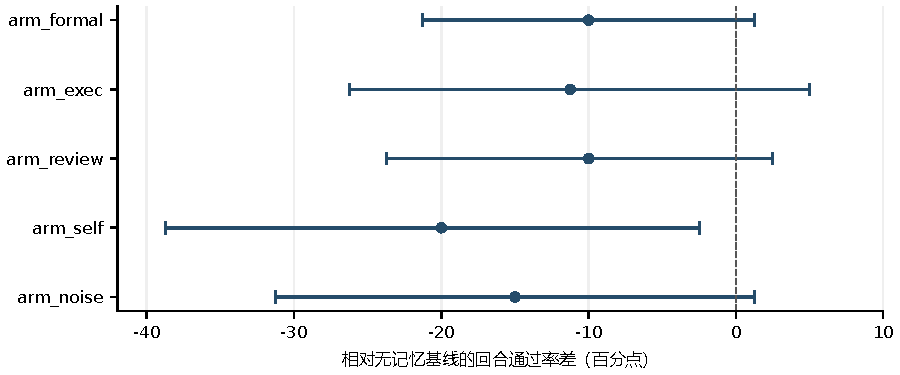
\includegraphics[width=\linewidth]{figures/generated/ch04-e02-effects.pdf}
\end{minipage}

\caption{验证层级与实际操作分开呈现。上方为综述的定性框架\cite{rsi-survey-2607}；
下方点与线段分别表示 E02 各记忆臂相对无记忆基线的通过率差和历史 95\% 题级自助区间。
数值来自表~\ref{tab:ch04-e02}，以百分点呈现；每臂 \measured{16} 题、每题 \measured{5} 个回合。
区间含零不表示等价，臂间差异应直接比较。此图保留旧估计，不替代完整验证层级的检验。}
\label{fig:ch04-ladder}
\end{figure}


\subsection{本轮的边界}
\label{sec:ch04-limits}

当前记录支持对六种已实现方案作描述，并提供反馈管道的故障案例。
它不支持“形式验证一定优于自评”，也不支持反方向的普遍断言。
新实验应重新冻结信息可见范围、反馈原文归档、任务内工具许可和成本口径，使用新运行标识。
旧轨迹不能因代码修复而被重新命名为新设计的观测。
E02b 与候选 P8 尚未执行，作为十个研究问题之外的扩展方向保留。

\section{反馈通道的相关错误：多看一眼为什么未必多一份证据}
\label{sec:ch04-correlated}

把作答者与评审者分成两个组件，是一种有用的结构安排，但组件数量不等于证据来源数量。两个请求若使用相同模型、相同材料、相近的提示，可能共同忽略同一处契约，也可能因为重新组织任务而发现不同问题。哪种情况占主导需要检查，不能由“独立评审”这个名字决定。

Reflexion 将行动、评估和语言反思分成不同角色，再把反思用于后续尝试；Self-Refine 则明确使用同一模型生成、反馈与修订\cite{reflexion-2303,self-refine-2303}。这些工作提供了不同的流程组织方式，不能仅凭角色图推断错误统计上独立，更不能把某项任务上的收益保证移植到任意模型与环境。

\subsection{相同模型、不同提示与独立证据是三个概念}

在 E02 中，评审提示把输入称作提交者的代码，自评提示把输入称作刚完成的代码。两者都通过同一个后端发起一个新请求；按保留实现，传入题目及含测试源码的文件渲染文本。自评请求没有继续原来的对话，也没有读取生成者的隐含状态。因而本次比较最多涉及这两类提示及其完整下游流程，不能声称隔离出了“他人判断”和“亲历者反思”的差异。

若要研究上下文影响，可以固定同一提交，比较只给代码、给完整执行轨迹、给截取的关键观察三种输入。若要研究评审模型差异，则应保持输入构造一致，再改变评审者。两项因素同时改变时，得到的是完整配置差异，仍有工程价值，但归因范围必须随之收窄。

更换模型也不自动消除相关错误。不同模型可能共享训练材料，面对同一缺失规格也都无法判断；同一模型在看到真正新增的测试反例后，反而可能修正先前错误。因此，应追踪新增了什么证据，而不只记录换了哪个名称。对栈案例而言，增加一个同样声称“逻辑正确”的评审不如实际检查一次状态变化；这是一种针对本例的诊断选择，不是所有任务都优先运行测试的定律。

\subsection{多数票需要先查共同盲点}

如果若干评审都读到同一份不完整材料，多数票可能只是在重复材料的偏差。例如题目要求“不修改调用者传入的列表”，评审输入却只保留返回值说明。多数评审都赞成原地修改，不能补回被删除的要求。这里应修复输入，而不是增加投票次数。

检查共同盲点可以从错误集合开始。对同一批候选分别保存各评审的判断，看看它们在哪些样本上同时失误、在哪些样本上互补。总准确率相近的评审，错误重叠可能很不同；总准确率较低的评审，也可能对某个关键风险提供独有证据。但选择评审组合的过程本身会使用数据，最终效果应留给未参与选择的材料检验。

如果只保存合并后的多数标签，后续就无法区分多数一致与少数异议，也不能检查仲裁是否压掉了有效反例。实际归档可保留每份意见、输入版本及合并规则，把合并结论作为派生结果。这样发生争议时，可以回到具体哪项证据被忽略，而不是重新让模型表决一次。

\subsection{理由相同不等于证据充分，理由不同也不等于相互独立}

语言表面上的多样性很容易误导。几位评审分别说“需要处理边界”“容器状态不正确”“可能有副作用”，可能都只是泛泛重述题目；一位评审说“长度没有减少”，另一位说“旧末项仍能再次读到”，却可能是在描述同一个可执行事实。评价互补性应落到观测与覆盖条件，而不是统计用了多少不同词语。

生成反馈时要求给理由，有助于让判断可审查，却不保证理由真实反映判断过程。因此，本书把理由视为一个待检验的文本产物。能核对它是否与代码和观察相容，能检查按它行动的效果；不能因为理由写得详细，就宣称已经测量了模型的真实因果机制。

这也解释了为什么“让模型更认真地反思”通常不是完整的实验操作。认真是一种提示措辞，可能改变长度、生成成本、关注点和回答风格。若预期收益来自更好的错误定位，就应记录定位是否更具体、更准确以及是否改善修复，而不只检查输出是否更长。

\subsection{信息冲突比一个错误标签更复杂}

E02 噪声臂提供了具体例子。实现翻转开头的验收判定后，仍附未改变的测试输出。当标题说失败而输出显示通过时，模型面对的是两条互相冲突的线索；它可以信标题、信日志，也可以编出第三种解释来调和冲突。这三种反应不同于在只有一个标签时被错误告知结果。

归档经验中确实出现了“本地测试全绿仍可能验收失败”和“公开测试全过不代表验收通过”的解释。这些文字来自被翻转标签的记录，并非我们事后杜撰；但它们也没有证据证明另有一个更严格的验收器实际失败。对不一致输入作合理化解释，是本例可见的风险。至于这些解释是否造成后续失分，还需要看检索和实际修改，不能由一句话直接判定。

若下一轮研究纯标签噪声，就只提供预先定义的标签，避免同时泄露原标签；若研究矛盾信息下的处理，则应把标题与日志的冲突作为独立因素，记录系统如何仲裁。若研究日志隐藏，除了删除总结行，还要考虑断言回溯、错误标记、用例名称和期望值。不同目的需要不同的遮蔽规则，不能用同一个“无判定”名称混合。

\subsection{反馈源的可信度需要具体到命题}

编译器可以可靠地告诉我们某种语言规则是否被接受，却不能因此替代产品需求的判断。测试可以指出一个输入上的输出错误，却未必覆盖性能与隐私约束。用户的纠正可以澄清其意图，但若不同用户有不同目标，就需要保留身份与任务上下文，而不是合成一个全局偏好。

因此，更有用的问题是“这个来源支持哪个命题、在什么条件下支持”，而不是给来源贴一个永远有效的可信等级。形式检查同样需要规格与检查器的假设；若证明的是一个写错的规格，证明正确也不会使产品满足真实需求。验证层级提示我们关注信号与外部约束的联系，不能让我们跳过被检查对象本身。

\section{迟到反馈：结果到达时，系统已经换了版本}
\label{sec:ch04-delay}

编程小题通常很快返回测试结果，用户复核、异步任务和业务结果却可能晚得多。反馈到达时，候选代码、记忆或工具版本已经改变。第\ref{ch02}章给出的版本与事件关联，解决的是把结果接回实际执行对象；本节进一步处理时间顺序怎样改变反馈的可用信息与评价分母。以下是设计示例，不是新增实测。

\subsection{按可用时刻释放反馈}

动作发生、反馈生成、系统接收是三个时刻，分别确定谁执行了动作、检查何时完成，以及更新器从什么时候起可以利用结果。离线重放若按任务开始时间排序，并在每题结束后立即写入后来才取得的全部结果，就给系统增加了当时不知道的知识。评价真实延迟下的在线更新，应按反馈可用时刻释放信息；评价标签齐备后的批量学习，则另行定义离线流程。

时间记录还需注明时区与时钟来源。不同服务未必同步，毫秒级字符串不保证毫秒级可比性。若只能确认先后顺序，就保存事件序列与时间范围，不据此推断更精确的因果顺序。

\subsection{旧失败先关联，再检查当前版本}

设候选甲处理任务后，系统已经切换到乙，随后才收到甲的失败结果。先用运行、输入与反馈请求标识找到甲的实际提交，再检查同一条件是否仍存在于乙。甲乙共享故障组件，旧反馈仍可能是有效警报；乙已修复该路径，直接回退反而可能恢复缺陷。对不能及时重现的外部故障，可以增加观察或限制相关动作，同时保留原因未定的状态。

相同题目可能在不同版本与权限下执行多次，不能仅凭题目文本关联。回调重复投递时，去重键应指向检查事件；相同的“验收失败”文字也可能来自两个真实任务。找不到原运行的反馈进入待核对区。检查器后来修错时，旧判定、修正及原因均应保留，才能解释系统当时为何采取某项更新。

接收、关联、诊断与经验发布还需能跨进程重启恢复，避免重复消费或正文与索引只写入一半。具体状态转换沿用第\ref{ch02}章的候选与发布约束；检验它们可在离线副本中于写入前后中断，检查是否丢记录或重复计数。这类故障注入验证反馈管道，不测量Agent能力。

\subsection{等待窗口也是评价条件}

旧版本的迟到失败不应混入新版本通过率；只统计新版本已经返回的快速成功，又可能高估它。报告需固定等待窗口，分别列出已返回的成功、已返回的失败和尚未返回，并说明各项分母及截尾处理。短期检查较易发现格式和接口错误，长期反馈可能揭示状态泄漏、维护负担或用户是否采用结果；较晚的结果也更容易受其他改动影响，不能一律称为更真实。

可以把近端指标用于快速筛查，再用较晚结果检验其代理关系。例如，测试通过是发布门槛，后续错误报告补充覆盖，两者保持各自分母。若将延迟结果回分配为早先动作的奖励，还需说明对应假设。经验的证据状态也保留时间线：先记“暂时通过已知检查”，观察窗口结束后再更新，避免把后来的确认倒填为当时已经确证。

\section{把下一轮反馈实验设计成能够回答的问题}
\label{sec:ch04-design}

发现旧设计的限制以后，最容易做的事是扩大题数，再跑一遍同样的装置。这样可能缩小某些区间，却不会把单元测试变成形式证明，也不会让两种角色提示成为两种独立信息源。下一轮应先决定要回答哪一个问题，再选择保留哪些差异、固定哪些条件。

下面给出一个尚未运行的设计框架。它不修改历史 E02 的协议身份，也不预先宣告能够判决 P2b。目的在于把“反馈有没有帮助”拆成规模与成本都可以说明的具体比较，避免一次试验承载互相冲突的解释。

\subsection{先区分固定提交的修复与连续任务的学习}

固定提交设计以候选代码为实验输入。每份代码在分配反馈之前已经确定，错误类型与初始质量不随反馈臂改变。不同修复者接收同一任务、同一提交、同一资源上限，只在指定反馈部分有差别。主要结果可以是修复后的独立检查通过率，辅助结果包括新增故障、调用量与修改范围。

这种设计的优点是容易追踪反馈作用于哪份代码；限制是它不研究系统怎样形成自己的错误分布。若实际部署中某种反馈会改变后续作答策略，固定提交比较就没有覆盖这种连锁影响。因此，固定提交适合诊断反馈组件，连续任务适合评估完整更新流程，二者可以前后衔接，不能互相替代。

连续任务设计让经验按时间进入记忆，测的是整个任务流中的表现。它需要冻结任务顺序或随机化规则、反馈到达规则、写入器、检索器、预算与起始状态。若某臂提前成功从而少写经验，这也是流程的一部分，不能事后强行补足相同条数而不计成本。分析单位还应覆盖经验共享造成的依赖：同一条任务流内的回合不能轻率地当作完全独立样本。

两种设计可以共享任务来源，但用于选择方案的数据和最终确认数据应保持用途边界。先用小规模固定提交诊断格式、输入与修订分支，再冻结连续任务方案，能够减少把工程故障误当理论负结果的风险。诊断阶段得到的分数仍应完整保存，不能挑出最好看的配置后把它称作未经选择的结果。

\subsection{把反馈操作写成输入差异表}

每一臂至少说明：是否见到测试源码，是否见到执行结果，是否见到明确标签，是否见到模型解释，是否继承原轨迹，以及反馈何时交给执行者。这些字段共同决定实际信息边界。只填“外部反馈”或“内部反思”无法让另一个实现者复现比较。

如果比较标签与诊断文本，可以让两臂都看到相同标签，只增加诊断内容；如果比较执行输出与模型意见，则必须明确模型意见是否已经读过输出，否则“意见”可能只是对同一输出的压缩。若要研究没有外部检查的自评，应核查题目附件、测试源码、缓存记忆和提示模板是否已经传入检查结果。

信息量与成本有时无法同时完全匹配。完整日志比一行标签长，模型读它需要更多输入；压缩日志又引入压缩器的选择。可以明确比较等调用上限、等总成本或实际配置三种不同问题，选择其中一种作为主要口径，再报告其他资源。不能把同样的回合预算说成所有环节资源相等。

\subsection{反馈档案应支持回放，也应支持否认过强结论}

每份反馈保存原始输入与原始输出，并保留经过截断、脱敏或格式修复后的实际展示版本。模型看到的是展示版本，审计需要知道它与原文差在哪。若只保存原文，无法确认被截掉的部分是否正好包含关键断言；若只保存摘要，无法核对摘要是否歪曲了原意。

不同权限下可以保存不同级别的材料，但缺失必须显式记录。敏感内容不宜为复现而无限复制；可在受控位置保留原文，在分析中使用引用与必要摘要。无论选择哪种方案，都不能在报告中声称记录了实际上没有保存的字段。E02 的中间模型评审原文缺失，就使逐字诊断审计受到限制；保留这个限制比事后重跑生成一段相似文字更诚实。

运行标识还需要绑定实际代码，而不仅是仓库当前提交号。E02 配置中的提交号早于其运行器进入版本库，现存代码与稍后首次提交一致，但缺少运行时的未提交差异与完整源码指纹。这不使所有轨迹失效，却限制了“逐字复现原运行实现”的承诺。新设计可以保存必要代码快照与配置散列，使之后的修复不会模糊旧实验身份。

\subsection{门槛、缺失与比较数量要在结果出现前说明}

诊断比较应预先定义主要结果和最小有用变化，并说明失败、超时、格式错误如何入账。格式错误既可能是接口不适配，也可能影响实际部署效用；若工程问题修复后重跑，应使用新版本和新记录，不能只替换旧数据中的失败行。报告可以同时给出完整方案表现与预定条件下的内容分析，前提是分母与选择规则清楚。

多个反馈臂之间可以产生许多两两比较。若看到结果后只挑一个有利差值，单个区间就不再代表整个选择流程的不确定性。主要比较应提前指定，探索性比较另列；需要联合判断完整排序时，还应考虑比较数量和方向约束。相邻两个点估计反序仅是描述，不能单独作为整条层级被推翻的判据。

样本规划还要考虑错误提交的构成。如果样本大多是已经正确的代码，评审者总说通过也可能获得高标签准确率，却没有展示定位失败的能力。可以报告成功与失败候选各自的判定表现，并按预定目标分布汇总。人为平衡样本便于机制检查，但总体指标应注明这种抽样，不能直接当成部署环境中的错误率。

\subsection{用停止规则保护问题本身}

工程试跑可以设置明确的停止条件：归档字段缺失、工具许可与声明不一致、任务材料越过信息边界，或账本不能闭合时，先停止扩大规模并修复。停止是为了保持实验身份，不能只在结果不好时启用。正式试验中的统计停止规则则另行规定，避免反复查看区间后在恰好有利的时刻收工。

最终报告应回答三个层次的问题：实际执行了什么配置，这批数据呈现了什么差异，这个差异支持原问题到哪一步。若第三层仍不能回答，可以保留有效的工程与机制发现，并明确待补设计。第16章的研究问题表将已有观察连到后续对照，每项试验按自己能够回答的问题报告。


\section{条件变化：先定位断点，再选择改动}
\label{sec:ch04-conditions}

如果结果标签本身与独立检查频繁冲突，先检查规格、环境和判定来源。
如果标签一致而诊断偏离证据，改进诊断输入或约束；如果诊断正确但未触发行动，检查执行与预算。
如果当前题修好而后续题受损，则查适用条件、检索和发布门槛。
这些分支可以并存，不能用一个低标签不一致率排除全部上游问题。

族间方向不同，提示应补充按族报告和任务分布分析；总体平均值仍可回答既定目标分布下的平均表现。
测试反复进入更新环节时，应保留独立检查，必要时按冻结方案扩展覆盖；轮换也会改变难度，不能把分数变化直接当进步。
在没有执行反馈的领域，仍可寻求可核对的原文、外部记录或人工纠正，并说明其滞后、主观性与覆盖范围。

\begin{principlebox}
先建立观察与候选版本的对应关系，再判断反馈值不值得写入。
标签一致性、诊断有效性、行动执行和迁移收益各自需要证据。
定性层级帮助提出比较，实际输入与实现决定比较究竟测到了什么。
样本规划不替代操作有效性；一次负结果也不自动提供负结果的原因。
\end{principlebox}

\section{非可验证前沿：方向生成在层级之前}
\label{sec:ch04-framing}

层级索引的是\textbf{方向评估}：给定一个候选方向，判断它是否成立、是否值得投入。
它不索引\textbf{方向生成}：哪些问题值得被评估，
以及何时一个仍被高分评价的问题已经不值得回答\cite{rsi-survey-2607}。
方向生成在逻辑上\textbf{先于}层级，不是层级的一级。

一个闭环可以爬到层级顶端、保持一个诚实的评估器、
检测到自己的代理指标被腐蚀，却仍然在一个早该放弃的问题上做得很好——
\textbf{因为层级把“问题”当作给定的}。
这类失效（原文称为 frame lock-in）的诊断难点在于观察边界：
前三类失效（自证循环、塌缩、多样性塌缩）
可能在内部指标上留下线索，而目标是否值得优化往往还需外部需求来判断\cite{rsi-survey-2607}。

把这条放回本章的实验：
E02 的六个臂都在回答同一批给定的 \measured{16} 道题，
这些比较也答不了“这 \measured{16} 道题值不值得被回答”。
这是第 16 章要处理的问题，本章只把边界划出来。

% ---------- 6. 反例 ----------
\begin{pitfallbox}
\textbf{把后来正确的解释，倒填成当时正确的行动。}
栈案例中的经验正确指出删除操作缺失，但原回合已经结束。复述经验不能改变提交记录。

\textbf{把相同臂名，当作相同信息边界。}
自评提示声称没有测试结果，并不意味着它没有测试源文件；新建上下文也不等于拥有独立判断来源。

\textbf{把接近的调用数，当作完整成本相同。}
六臂调用数依次为 \measured{431}、\measured{403}、\measured{406}、\measured{408}、\measured{409}、\measured{407}。
这些总数已含记忆生成和模型评审的旁路调用，不应再把 \texttt{side\_calls} 加一遍。
账本中每臂约 \measured{332}--\measured{385} 秒是回合计时之和，未完整包含旁路调用等耗时，不能称为各臂端到端墙钟。
\end{pitfallbox}

\section*{习题}
\begin{enumerate}[label=4-\arabic*.,ref=4-\arabic*]
  \item\label{ex:ch04-1} 表~\ref{tab:ch04-six} 的六类信号是代码特有的。
        为你熟悉的一个非编程 Agent 场景（检索问答、数据分析、流程自动化）
        补出对应的六类信号，并标出其中哪几类可重放。
  \item\label{ex:ch04-2} 本章区分“反馈标签一致性”和“迁移收益”。
        请构造一个例子，使得标签不一致率为 0 而收益为负（提示：想检索环节），
        再构造一个使标签不一致率高而收益为正的例子。
  \item\label{ex:ch04-3} 表~\ref{tab:ch04-adj} 按旧臂顺序出现一次点估计反序（执行输出 vs 评审提示，
        点估计 \measured{$-0.0125$}）。
        请列出三种能产生这种反转的\emph{设计}原因（不是“真实就是这样”），
        并说明各自应当如何被排除。
  \item\leavevmode\label{ex:ch04-4}E02 已有 \measured{16} 道配对题，区间精度公式给出约 \calcnum{592} 道独立题的规划示例。
        扩题、增加每题重复次数、改用分层估计，分别处理哪种不确定性？
        为什么后两项不能直接算作增加了独立题数，这个规划数又为什么不是功效保证？
  \item\label{ex:ch04-5} 第 \ref{sec:ch04-framing} 节说方向生成先于层级。
        设计一个可观测量，使得“一个闭环正在优化一个不值得优化的目标”这件事变得可检测。
\end{enumerate}

\section*{常见误解}
\begin{itemize}
\sloppy
  \item \textbf{“反馈越可靠，收益越高”。}
        E02 中有四臂各自的 \measured{8} 条训练标签都与验收一致。其中两臂的标签直接取自验收结果或退出码，另两臂来自模型评审或自评。到了封存题，四臂的通过率点估计均低于无记忆基线，只有自评臂的差值区间完全低于零（表~\ref{tab:ch04-e02}）。
  \item \textbf{“E02 说明验证层级是错的”。}
        本轮的反馈操作并未覆盖完整概念层级，且样本与确认性设计仍有缺口，本轮不能由该排序推出完整反馈层级的规律。
        区间包含 0 与一次反转都只作为读数，不构成判决。
  \item \textbf{“有了测试就有接地，自进化就能跑起来”。}
        固定基准存在过拟合与投机风险\cite{rsi-survey-2607}；
        接地需要维持独立检查及适当覆盖；轮换与留出检验须按协议进行，也不能代替对规格的核对。
  \item \textbf{“第 4 层最便宜，所以从它开始最划算”。}
        原综述将其概括为低成本、易投机的信号\cite{rsi-survey-2607}，并未给出适用于所有任务的费用排序。
        自一致性可能需要多次采样，执行一个简单断言也可能很便宜；成本与失效风险均须按具体流程测量，不能从定性层级直接推出部署策略。
\end{itemize}

\section*{进一步阅读}
\begin{itemize}
\sloppy
  \item \cite{rsi-survey-2607}：验证层级四层（\S 5.2）、包含frame lock-in在内的四类失效模式（\S 5.3）、
        方向生成与方向评估之分（\S 5.4）的出处；
        本章表~\ref{tab:ch04-hier} 与 \S\ref{sec:ch04-framing} 采用其概念讨论。
        读它时务必保留原文那句"not a measured law"。
  \item \cite{coding-survey-2608}：六类代码特有信号 E/D/T/R/Q/H 与 Figure 7 的占比统计，
        本章表~\ref{tab:ch04-six} 的数字来源；\S 4.1 的边界判据（学习信号必须来自自身尝试）
        是第 1 章 1.1 的另一处依据。
  \item \cite{ksi-2607}：带适用条件的知识条目（\texttt{applies\_when} /
        \texttt{does\_not\_apply\_when}），本章 \S\ref{sec:ch04-hypothesis} 的设计规则来源。
  \item 本书第 3 章：配对差、重采样单位与 MDE 的口径；
        第 14 章：评审者本身成为优化目标时（自证循环）会发生什么；
        第 16 章：方向生成与 frame lock-in 的最终处理。
\end{itemize}
